
\clearpage









\section{Abstract}


\tmpsection{One or two sentences providing a basic introduction to the field}
% comprehensible to a scientist in any discipline.
\lettr{A}n increasingly large fraction of emerging diseases come from animals \cite{jones2008global, taylor2001risk} and these diseases have a huge impact on human health.
The chance that a new disease will come from any particularly wild host species increases with the diversity of pathogens in that species.
However, the factors that control pathogen diversity in wild populations are still unknown.



\tmpsection{Two to three sentences of more detailed background}
Population density is known to increase pathogen richness while theory suggests that population structure may also play a role.
However, these factors, along with population abundance, are intrinsically linked; reducing density reduces contacts between individuals.
In group living species, this is particularly true, with group size and the number of groups and distribution size contributing to total animal density. 
As these factors are completely interdependant, it is very difficult to study them empirically e.g. in a comparative frame work.

\tmpsection{One sentence clearly stating the general problem (the gap)}
% being addressed by this particular study.

It is unknown whether it is specifically density that controls pathogen diversity or whether density merely correlates with population structure, group size or population size (abundance).


\tmpsection{One sentence summarising the main result}
%  (with the words “here we show” or their equivalent).
Here I use metapopulation SIR models to test whether it is density \emph{per se} that increases the ability of a new pathogen to invade as apposed to colony size, population abundance or population structure.



\tmpsection{Two or three sentences explaining what the main result reveals in direct comparison to what was thought to be the case previously}
% or how the main result adds to previous knowledge



\tmpsection{One or two sentences to put the results into a more general context.}

\tmpsection{Two or three sentences to provide a broader perspective, }
% readily comprehensible to a scientist in any discipline.





%%%%%%%%%%%%%%%%%%%%%%%%%%%%%%%%%%%%%%%%%%%%%%%%%%%%%%%%%%%%%%%%%%%%%%%%%%%%%%%%%%%%%%%%%%%%%%%%%%%%%%%%%%%%%%%%%%%%%%%%%%%%%%%%%%%%%%%%%%%%%%%%%%%%%%%%%%%

\clearpage
\section{Introduction}

%%%%%%%%%%%%%%%%%%%%%%%%%%%%%%%%%%%%%%%%%%%%%%%%%%%%%%%%%%%%%%%%%%%%%%%%%%%%%%%%%%%%%%%%%%%%%%%%%%%%%%%%%%%%%%%%%%%%%%%%%%%%%%%%%%%%%%%%%%%%%%%%%%%%%%%%%%%




\subsection{General Intro}
%%%%%%%%%%%%%%%%%%%%%%%%%%%%%%
% A basic introduction to the field,
% comprehensible to a scientist in any discipline.


\subsubsection{Why is pathogen diversity important?}


\subsubsection{We know some factors that correlate with pathogen diversity}


\subsubsection{But we do not understand the mechanistic processes}







\subsection{Specific Intro}
%%%%%%%%%%%%%%%%%%%%%%%%%%%%%%
% more detailed background}
% comprehensible to scientists in related disciplines.




\subsection{The gap}
%%%%%%%%%%%%%%%%%%%%%%%%%%%%%%


\subsection{What I did}
%%%%%%%%%%%%%%%%%%%%%%%%%%%%%%


\subsection{What I found}
%%%%%%%%%%%%%%%%%%%%%%%%%%%%%%
% One sentence summarising the main result
% (with the words “here we show” or their equivalent).


%%%%%%%%%%%%%%%%%%%%%%%%%%%%%%%%%%%%%%%%%%%%%%%%%%%%%%%%%%%%%%%%%%%%%%%%%%%%%%%%%%%%%%%%%%%%%%%%%%%%%%%%%%%%%%%%%%%%%%%%%%%%%%%%%%%%%%%%%%%%%%%%%%%%%%%%%%%

\clearpage
\section{Methods}

%%%%%%%%%%%%%%%%%%%%%%%%%%%%%%%%%%%%%%%%%%%%%%%%%%%%%%%%%%%%%%%%%%%%%%%%%%%%%%%%%%%%%%%%%%%%%%%%%%%%%%%%%%%%%%%%%%%%%%%%%%%%%%%%%%%%%%%%%%%%%%%%%%%%%%%%%%%

%%




\subsection{Metapopulation model}




\subsubsection{Two pathogen SIR model}

We examine a multpathogen SIR model. 
This is a compartment model with individuals being classed as susceptible, infected or recovered with immunity (Figure~\ref{f:sir}).
Susceptible individuals are counted in class $S$.
There are three infected classes, $I_1$, $I_2$ and $I_{12}$, being individuals infected with pathogen 1, pathogen 2 or both respectively.
Recovered individuals, $R$, are immune to both pathogens, even if they have only been infected with one.
Furthermore, recovery from a pathogen moves an individual straight into the recovered class, even if the individual is infected with both pathogen.
This modelling choice allows the model to be easily expanded to included more than two pathogens.
The assumption of immediate recovery from all other diseases is likely to be quite accurate for very closely related pathogens as is being studied here as once an acquired immune response is activated, all infections are likely to be cleared quickly.

The coinfection rate is adjusted compared to the first infection rate by a factor $\alpha$.
Birth and death rates are assumed to be equal, $b = d$.


\subsubsection{Metapopulation}


The population is divided into a number of subpopulations.
This metapopulation is modelled as a network with subpopulations being nodes and dispersal between subpopulations being indicated by edges (Figure~\ref{f:net})
Individuals with a subpopulation interact randomly so that the subpopulation is fully mixed.
However, dispersal between subpopulations occurs at a rate $\lambda$.
Individuals can only disperse to subpopulations connected to theirs in the network.
The rate of dispersal is not affected by the number of edges a subpopulation has (the degree of the subpopulation).
So the dispersal rate from a subpopulation $m$ with degree $k_m$ to subpopulation $n$ is $\frac{\lambda}{k_m}$.
Note this rate is independent of the degree of subpopulation $n$.





\subsubsection{Stochastic simulations}

We examine this model using stochastic, continuous time simulations using the Gillespie algorithm.
At each step in the simulation we calculate the rate that each possible event might occur.
One event is then randomly chosen, weighted by it's rate
\begin{align}
  p(\text{event } i) = \frac{r_i}{\sum_i r_i}
\end{align}
where $r_i$ is the rate that event $i$ occurs.
Finally, the length of the time step, $\delta$, is drawn from an exponential distribution 
\begin{align}
  \delta \sim \operatorname{Exp}\left(\sum_i r_i  \right).
\end{align}
This means that the length of each simulation is stochastic. 
We define the number of events we wish to simulate instead.


\begin{figure}[t]
\centering
  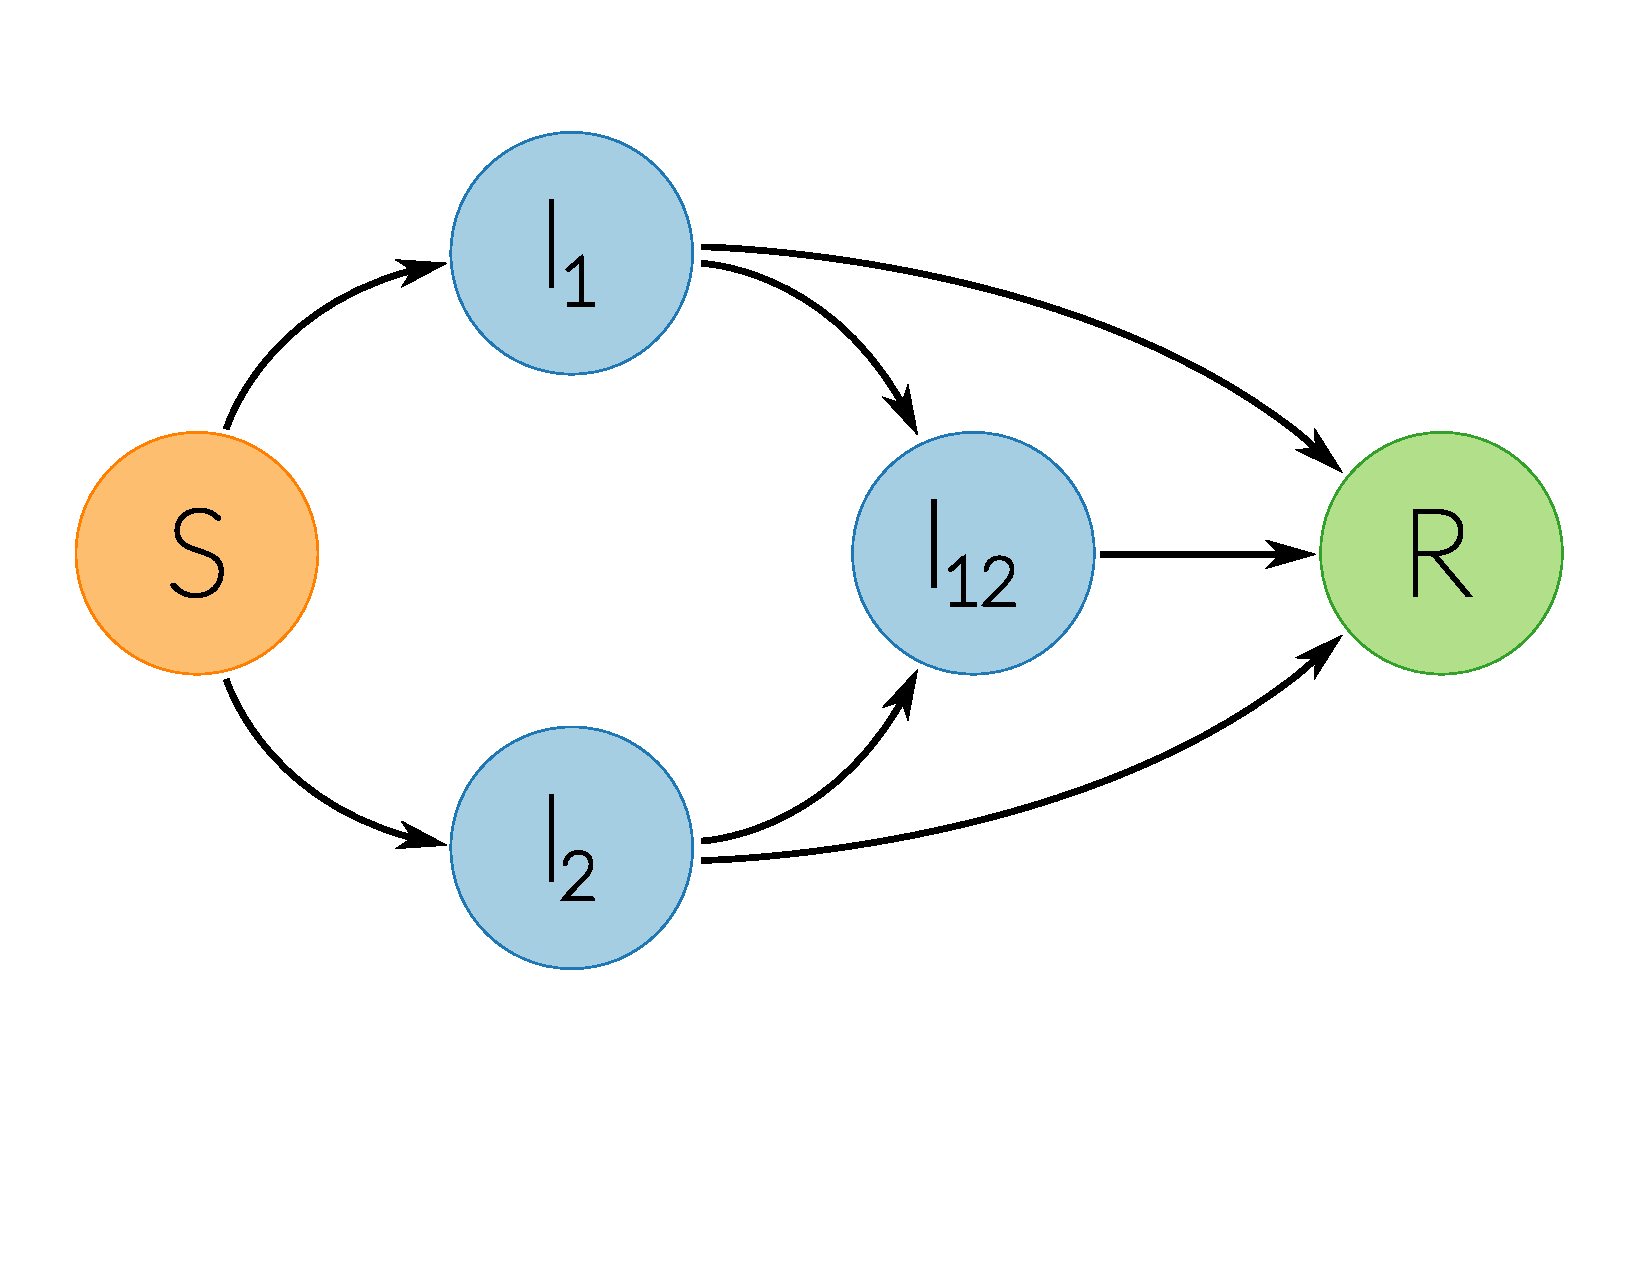
\includegraphics[width=0.4\textwidth]{imgs/SIRoption1.pdf}
  \caption{The SIR model used.}
  \label{f:sir}
\end{figure}


We can now write down the rates of all events. 
I define $I^+_p$ to be the sum of all classes that are infectious with pathogen $p$, for example $I^+_1 = I_1 + I_{12}$. 
Assuming asexual reproduction, that all classes reproduce at the same rate and that individuals are born into the susceptible class we get
\begin{align}
  P\left( S_{nt^\prime} = S_{nt} +1\right) &= b\left( S_{nt}+\sum_q I_{qnt} + R_{nt}\right) 
\end{align}
where $P\left( S_{nt^\prime} = S_{nt} +1\right)$ is the probability that the number of susceptibles in subpopulation $n$ will increase by 1 (a single birth) the short time interval $t$ to $t^\prime$ and $\sum_q I_{qnt}$ is the sum of all infection classes $q \in {1, 2, 12}$.
The rates of death, given a death rate $d$ are given by
\begin{align}
  P\left( S_{nt^\prime} = S_{nt}-1 \right) &= dS_{nt} \\
  P\left( I_{qnt^\prime} = I_{qnt}-1 \right) &= dI_{qnt}\\
  P\left( R_{nt^\prime} = R_{nt}-1 \right) &= dR_{nt}.
\end{align}
Infection of a susceptible with either pathogen 1 or 2, $S \rightarrow I_p$ where $p\in \{1,2\}$, is given by
\begin{align}
  P\left( I_{pnt^\prime} = I_{pnt}+1, S_{nt^\prime} = S_{nt}-1 \right) &= \beta S_{nt}I^+_{pnt},
\end{align}
while coinfection, given a crossimmunity factor $\alpha$, is given by
\begin{align}
  P\left( I_{12,nt^\prime} = I_{12,nt}+1,\: I_{pnt^\prime} = I_{pnt}-1\right) = \alpha\beta I_{nt}I^+_{pnt}.
\end{align}
The probability of migration from colony $m$ (with degree $k_m$) to colony $n$, given a dispersal rate $\lambda$ is given by
\begin{align}
  P\left(S_{nt^\prime}=S_{nt}+1,\: S_{mt^\prime} = S_{mt}-1\right) &= \frac{\lambda S_{mt}}{k_m-1}\\
  P\left(I_{qnt^\prime}=I_{qnt}+1,\: I_{qmt^\prime} = I_{qmt}-1\right) &= \frac{\lambda I_{qmt}}{k_m}\\
  P\left(R_{nt^\prime}=S_{nt}+1,\: R_{mt^\prime} = R_{mt}-1\right) &= \frac{\lambda R_{mt}}{k_m}.
\end{align}
Finally, recovery from any infectious class occurs at a rate $\gamma$
\begin{align}
  P\left( I_{qnt^\prime} = I_{qnt}-1,\: R_{nt^\prime} = R_{nt}+1 \right) &= \gamma I_{qnt}.
\end{align}







%%%%%%%%%%%%%%%%%%%%%%%%%%%%%%%%%%%%%%%%%%%%%%%%%%%%%%%%%%%%%%%%%%%%%%%%%%%%%%%%%%%%%%%%%
%%%% Constant density size. 
%%%%%%%%%%%%%%%%%%%%%%%%%%%%%%%%%%%%%%%%%%%%%%%%%%%%%%%%%%%%%%%%%%%%%%%%%%%%%%%%%%%%%%%%%







%%%%%%%%%%%%%%%%%%%%%%%%%%%%%%%%%%%%%%%%%%%%%%%%%%%%%%%%%%%%%%%%%%%%%%%%%%%%%%%%%%%%%%%%%
%%%% Constant density 2. 
%%%%%%%%%%%%%%%%%%%%%%%%%%%%%%%%%%%%%%%%%%%%%%%%%%%%%%%%%%%%%%%%%%%%%%%%%%%%%%%%%%%%%%%%%









%%%%%%%%%%%%%%%%%%%%%%%%%%%%%%%%%%%%%%%%%%%%%%%%%%%%%%%%%%%%%%%%%%%%%%%%%%%%%%%%%%%%%%%%%
%%%% Constant Population. 
%%%%%%%%%%%%%%%%%%%%%%%%%%%%%%%%%%%%%%%%%%%%%%%%%%%%%%%%%%%%%%%%%%%%%%%%%%%%%%%%%%%%%%%%%












In each simulation the population is seeded with 20 infected individuals of disease 1 in each colony. 
Disease 1 is then allowed to spread and reach equilibrium. 
After \ensuremath{7\times 10^{5}} events, 5 individuals infected with disease 2 are added to one colony. 
After another \ensuremath{3\times 10^{5}} events the invasion of disease 2 is considered successful if any individuals with disease 2 still remain.



\subsection{Dispersal}
%%%%%%%%%%%%%%%%%%%%%%%%%%%%%%

The values used for the independant variables are chosen to highlight the affects of these variables. 
Dispersal values are $\lambda = 0.1, 0.01$ and $ 0.001$ dispersals per individual per year. 
$\lambda = 0.1$ relates to individuals moving between colonies on average twice per lifetime. 
Therefore exclusively juvenile dispersal would have dispersal rates similar to this. 
Otherwise it relates to dispersal being a rare event with animals often staying in a colony for many years.
$\lambda = 0.01$ relates to 20\% of individuals dispersing once in their lifetime.
This value is therefore close to male-biased dispersal, with female philopatry. 
Finally, $\lambda = 0.001$ relates to 2\% of individuals dispersing in their lifetime.
This therefore relates to a population that does not habitually disperse.




\subsection{Network structure}
%%%%%%%%%%%%%%%%%%%%%%%%%%%%%%
The network structure is synthetically created to be either fully or minimally connected (See Figure~\ref{f:net}). 
10 subpopulations was selected as a trade off between computation time and a network complicated enough that structure might have an effect. 
This value is artificially small compared to wildlife populations. 



\subsection{Parameter selection}


The fixed parameters used are chosen to roughly reflect realistic wild bat populations. 
The death rate $d$ is set as 0.05 per year giving a generation time of 20 years.
The birth rate $b$ is set to be equal to $d$ so that the population size is stable.
The recovery rate $\gamma$ is set to 0.1 giving a average infection duration of 10 years. 
This is therefore a chronic infection. 
It is very difficult to directly estimate infection durations in wild populations.
But it seems that these infections might be long lasting \cite{}.

Cross immunity is set to 0.1 so that an individual infected with one disease is 90\% less likely to be infected with another.
This is a rather arbitrary value.
However, the model assumes complete cross immunity after infection.
Furthermore, the rationale of the model is that the invading species might be a newly speciated strain of the endemic species.
Therefore cross immunity is likely to be very strong.

The population size of each subpopulation is set to 3000. 
This is appropriate for many bat species \cite{jones2009pantheria}, especially the large, frugivorous \emph{Pteropodidae} that have been particularly associated with recent zoonotic diseases.


Three values of the transmission rate $\beta$ are used, 2, 5 and 10.
All simulations are run under all three transmission rates as this is such a fundamental parameter.
Given the recovery, birth and death rates we can calculate an approximation of $R_0$ that ignores spatial structure.
That is, this is $R_0$ for the local, within-subpopulation dynamics.
Furthermore, it is $R_0$ for the first pathogen; $R_0$ of the invading pathogen will be lower due to competition.
We can calculate that $R_0 \approx \frac{\beta d}{d(d+ \gamma)}$.
For our three values of $\beta = 2, 5, 10$ we therefore get $R_0 \approx 13.3, 33.3, 66.6$.
These values are very high in part to again find a reasonable trade off between the number of simulations and the reasonableness of the parameters.
$R_0 \approx 13.3$ is similar to a highly contagious disease such as measles or pertussis. 


For the simulations where an invading pathogen is added to the populations the number of invading pathogens added is set to 10. 
This is a trade off between getting a reasonable proportion of invasions, while still retaining the stochastic nature of invasion.

For simulations studying extinction rates, half of the subpopulation were seeded with each pathogen.
2000 susceptibles and 1000 infected individuals were placed in each subpopulation in order to quickly reach equilibrium.











%%%%%%%%%%%%%%%%%%%%%%%%%%%%%%%%%%%%%%%%%%%%%%%%%%%%%%%%%%%%%%%%%%%%%%%%%%%%%%%%%%%%%%%%%%%%%%%%%%%%%%%%%%%%%%%%%%%%%%%%%%%%%%%%%%%%%%%%%%%%%%%%%%%%%%%%%%%

\clearpage
\section{Results}

%%%%%%%%%%%%%%%%%%%%%%%%%%%%%%%%%%%%%%%%%%%%%%%%%%%%%%%%%%%%%%%%%%%%%%%%%%%%%%%%%%%%%%%%%%%%%%%%%%%%%%%%%%%%%%%%%%%%%%%%%%%%%%%%%%%%%%%%%%%%%%%%%%%%%%%%%%%





\begin{knitrout}\footnotesize
\definecolor{shadecolor}{rgb}{0.969, 0.969, 0.969}\color{fgcolor}

{\centering 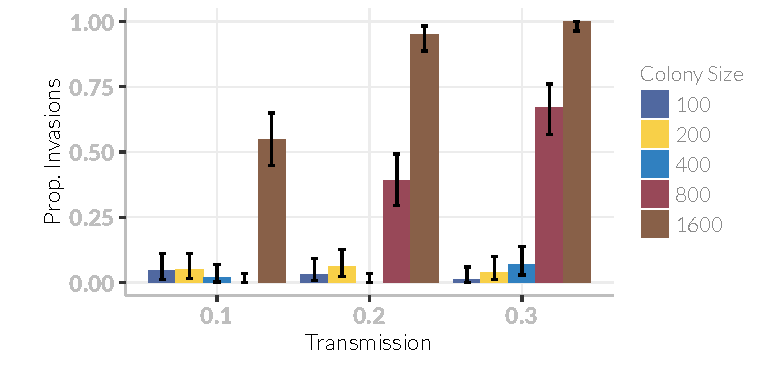
\includegraphics[width=0.8\textwidth]{figure/plotMeans-1} 

}




{\centering 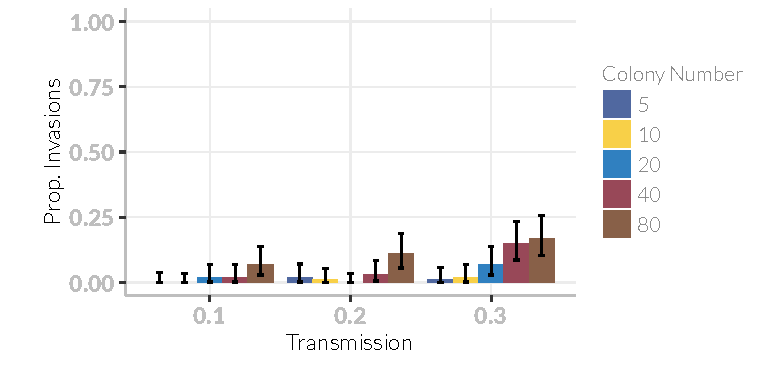
\includegraphics[width=0.8\textwidth]{figure/plotMeans-2} 

}




{\centering 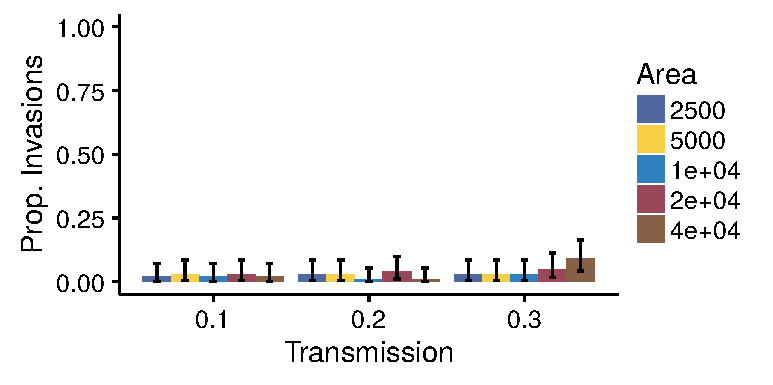
\includegraphics[width=0.8\textwidth]{figure/plotMeans-3} 

}



\end{knitrout}










\begin{knitrout}\footnotesize
\definecolor{shadecolor}{rgb}{0.969, 0.969, 0.969}\color{fgcolor}\begin{figure}[t]

{\centering 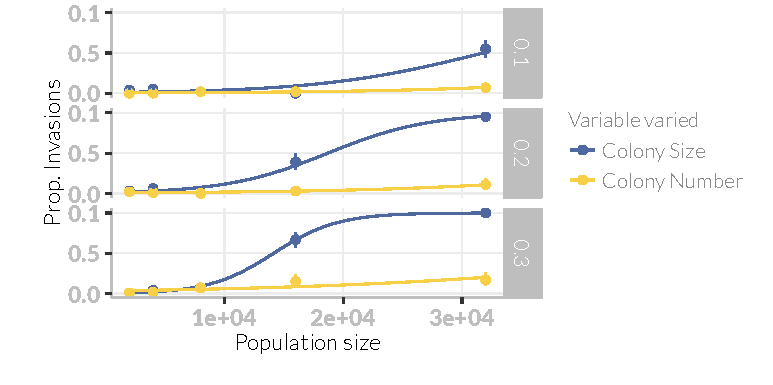
\includegraphics[width=0.9\textwidth]{figure/plotTransMeans-1} 

}

\caption[Comparison of the probability of invasion when population size is altered by changing colony size or colony number.]{
Comparison of the effect of population size on probability of invasion when population size is altered by changing colony size or colony number.
Relationship is shown seperately for each transmission value.
It can be seen that changes in colony size give a much greater increase in invasion probability thatn changes in colony number.
}\label{fig:plotTransMeans}
\end{figure}


\end{knitrout}





\begin{knitrout}\footnotesize
\definecolor{shadecolor}{rgb}{0.969, 0.969, 0.969}\color{fgcolor}\begin{figure}[t]

{\centering 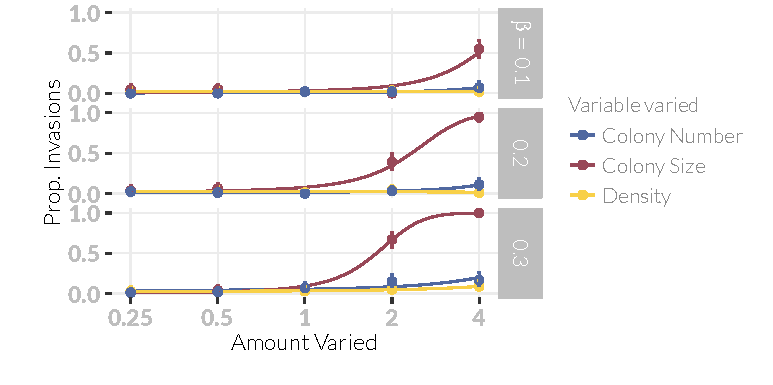
\includegraphics[width=\textwidth]{figure/plotValueChangeMeans-1} 

}

\caption[Comparison of the probability of invasion when population size is altered by changing colony size or colony number.]{
Relationship is shown seperately for each transmission value.
}\label{fig:plotValueChangeMeans}
\end{figure}


\end{knitrout}

%%%%%%%%%%%%%%%%%%%%%%%%%%%%%%%%%%%%%%%%%%%%%%%%%%%%%%%%%%%%%%%%%%%%%%%%%%%%%%%%%%%%%%%%%%%%%%%%%%%%%%%%%%%%%%%%%%%%%%%%%%%%%%%%%%%%%%%%%%%%%%%%%%%%%%%%%%%

\clearpage
\section{Discussion}

%%%%%%%%%%%%%%%%%%%%%%%%%%%%%%%%%%%%%%%%%%%%%%%%%%%%%%%%%%%%%%%%%%%%%%%%%%%%%%%%%%%%%%%%%%%%%%%%%%%%%%%%%%%%%%%%%%%%%%%%%%%%%%%%%%%%%%%%%%%%%%%%%%%%%%%%%%%

\subsection{Restate the gap and the main result}

Empirical studies on the role of population structure on the are equivocal and cannot examine the specific mechanisms by which pathogen communities are created and maintained.
I have used mechanistic, metapopulation models to test whether increased population structure can promote pathogen richness by facilitating invasion of new pathogens.



\subsection{Link results to consequences}

\subsubsection{Population structure does not affect pathogen richness}

Probably because dynamics are dominated by local processes.
This goes against many predictions that increasing $R_0$ increases pathogen richness.
Further work could examine reduced col  ony sizes to test when global structure become more important.
Measures of population structure should not be used to predict zoonotic potential.

\subsubsection{Dispersal does not affect pathogen richness}



\subsubsection{Network connectedness does not affect pathogen richness}

This is in direct contrast to \cite{campos2006pathogen}. 
However, the model in \cite{campos2006pathogen} is a contact network, so increasing the connectedness increases the chance of succesful transmission events for the first few transmission generations.
This lends support to the idea that I found now affect of connectedness due to the dominance of local dynamics.

Network connectedness can be seen as a function of average dispersal distance, density and colony size.
A high density species with small colony sizes must have colonies relatively close together.
Therefore colonies would be more likely to be connected for a given dispersal distance. 


\subsection{Discuss assumptions}

\subsubsection{Complete cross-immunity}

I have assumed that once recovered, individuals are immune to both pathogens. 
Furthermore, when a coinfected individual recovers from one pathogen, it immediately recovers from the other as well.
This is probably a fairly reasonable assumption given that I am modelling a newly evolved strain.
However, further work could relax this assumption using a model similar to \cite{poletto2015characterising} which contains additional classes for `infected with pathogen one, immune to pathogen two' and `infected with pathogen two, immune to pathogen one'.
The model here was formulated such that the study of systems with greater than two pathogens is still computationally feasible while a model such as used in \cite{poletto2015characterising} contains $3^\rho$ classes for a system with $\rho$ pathogen species.
This quickly becomes computationally restrictive.

\subsubsection{Identical strains}

Many papers on pathogen richness have focussed on the evolution of pathogen traits and have considered a trade off between transmission rate and virulence \cite{nowak1994superinfection, nowak1994superinfection} or infectious period \cite{poletto2013host}.
However, here we are interested in host traits.
Therefore we have assumed that pathogen strains are identical.
It is clear however that there are a number of factors that affect pathogen richness and our focus on host population structure does not imply that pathogen traits are not important.



%%%%%%%%%%%%%%%%%%%%%%%%%%%%%%%%%%%%%%%%%%%%%%%%%%%%%%%%%%%%%%%%%%%%%%%%%%%%%%%%%%%%%%%%%%%%%%%%%%%%%%%%%%%%%%%%%%%%%%%%%%%%%%%%%%%%%%%%%%%%%%%%%%%%%%%%%%%

\clearpage
\section{Appendix}

%%%%%%%%%%%%%%%%%%%%%%%%%%%%%%%%%%%%%%%%%%%%%%%%%%%%%%%%%%%%%%%%%%%%%%%%%%%%%%%%%%%%%%%%%%%%%%%%%%%%%%%%%%%%%%%%%%%%%%%%%%%%%%%%%%%%%%%%%%%%%%%%%%%%%%%%%%%

\begin{table}[b!]

\begin{tabular}{lp{5.6cm}p{4.3cm}l}
 & Explanation & Units&Value\\
\hline
$S$ & Susceptible individuals &&\\
$I_q$ & Infectious with diseases $q$ &&\\
$I^+_p$ & Sum of classes infected with pathogen $p$ &\\
$N$ & Number of colonies&& 10\\
$\bar{n}$ & Mean colony starting size && 3000\\
$\beta$ & Transmission rate & Transmission events per year per individual& 2, 5, 10\\
$\gamma$ & Recovery rate & Recovery events per year. & 0.1\\
$\lambda$ & Dispersal & Dispersal events per day per individual& 0.001--0.1\\
$b$ & Birth rate & Births per year per individual& 0.05\\
$d$ & Death rate & Deaths per year per individual & 0.05\\
$d_I$ & Infectious death rate & Additional deaths per day per individual&\\
$\rho$ & No. pathogens && 2\\
$p$ &  Pathogen index i.e. $p\in\{1,2\}$ for pathogens 1 and 2 & &\\
$q$ & Disease class i.e., $q\in\{1,2,12\}$&\\
$\mathcal{V}$ & Neighbourhood of a node &&\\
$t, t^\prime$ & Time and time plus waiting time i.e., $t+\delta$ & Days&\\
$k_i$ & Degree of node $i$ &&\\
$\delta$ & Waiting time until next event & Days&\\
$\alpha$ & Cross immunity & Proportion& 0.1\\
$n, m$ & Colony index &&\\
%$\bm{A}_{mn}$ & Adjacency matrix. & Distance &\\
$\mu$ & Maximum distance for edge to exist & km& 40, 100\\
$\sigma$ & Invading pathogen seed size & & 10\\
$r_i$ & The rate that event $i$ occurs. & Days$^{-1}$&\\
&&&\\
\end{tabular}
\caption{All symbols used.}
\label{t:params}
\end{table}




